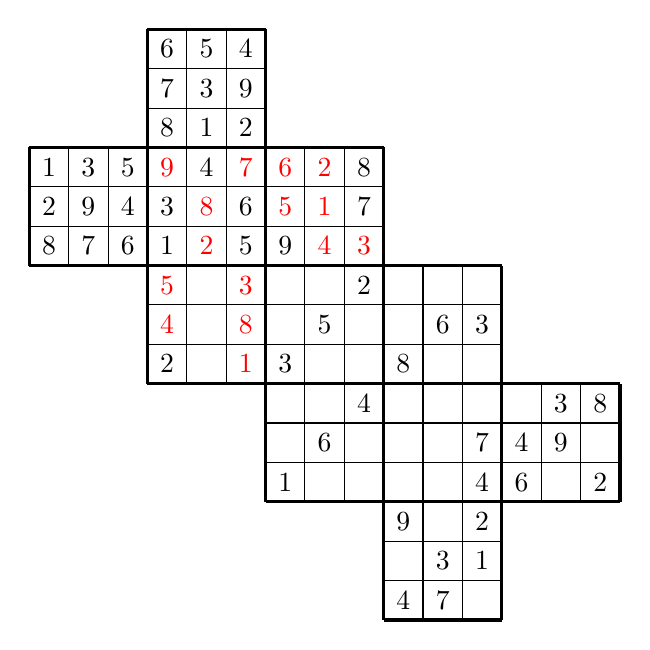
\begin{tikzpicture}[scale=0.5]

  \foreach \x/\y in {1/2,0/1,1/1,2/1,1/0,2/0,3/0,2/-1,3/-1,4/-1,3/-2} {
    \draw (3*\x,3*\y) grid (3*\x+3,3*\y+3);
    \draw[very thick, scale=3] (\x,\y) grid (\x+1,\y+1);
  }

  % Fill in block (2,1)
  \foreach \i/\j/\k in {4/1/1,4/2/3,4/3/5,5/1/2,5/2/9,5/3/4,6/1/8,6/2/7,6/3/6} {
    \node[anchor=center] at (\j-0.5, 9.5-\i) {\k};
  }

  % Fill in block (1,2)
  \foreach \i/\j/\k in {1/4/6,2/4/7,3/4/8,1/5/5,2/5/3,3/5/1,1/6/4,2/6/9,3/6/2} {
    \node[anchor=center] at (\j-0.5, 9.5-\i) {\k};
  }

  % Fill in block (2,2)
  \foreach \i/\j/\k in {4/4/\textcolor{red}{9},4/5/4,4/6/\textcolor{red}{7},5/5/\textcolor{red}{8},5/6/6,6/6/5,5/4/3,6/4/1,6/5/\textcolor{red}{2}} {
    \node[anchor=center] at (\j-0.5, 9.5-\i) {\k};
  }

  % Fill in block (2,3)
  \foreach \i/\j/\k in {4/9/8,5/9/7,6/7/9, 4/7/\textcolor{red}{6}, 4/8/\textcolor{red}{2}, 5/7/\textcolor{red}{5}, 5/8/\textcolor{red}{1}, 6/8/\textcolor{red}{4}, 6/9/\textcolor{red}{3}  } {
    \node[anchor=center] at (\j-0.5, 9.5-\i) {\k};
  }

  % Fill in block (3,2)
  \foreach \i/\j/\k in {9/4/2, 7/4/\textcolor{red}{5}, 8/4/\textcolor{red}{4}, 7/6/\textcolor{red}{3}, 8/6/\textcolor{red}{8}, 9/6/\textcolor{red}{1} } {
    \node[anchor=center] at (\j-0.5, 9.5-\i) {\k};
  }

  % Fill in block (3,3)
  \foreach \i/\j/\k in {7/9/2,9/7/3,8/8/5} {
    \node[anchor=center] at (\j-0.5, 9.5-\i) {\k};
  }

  % Fill in block (3,4)
  \foreach \i/\j/\k in {9/10/8,8/11/6,8/12/3} {
    \node[anchor=center] at (\j-0.5, 9.5-\i) {\k};
  }

  % Fill in block (4,3)
  \foreach \i/\j/\k in {12/7/1,11/8/6,10/9/4} {
    \node[anchor=center] at (\j-0.5, 9.5-\i) {\k};
  }

  % Fill in block (4,4)
  \foreach \i/\j/\k in {11/12/7,12/12/4} {
    \node[anchor=center] at (\j-0.5, 9.5-\i) {\k};
  }

  % Fill in block (4,5)
  \foreach \i/\j/\k in {10/14/3,10/15/8,11/13/4,11/14/9,12/13/6,12/15/2} {
    \node[anchor=center] at (\j-0.5, 9.5-\i) {\k};
  }

  % Fill in block (4,5)
  \foreach \i/\j/\k in {13/10/9,15/10/4,14/11/3,15/11/7,13/12/2,14/12/1} {
    \node[anchor=center] at (\j-0.5, 9.5-\i) {\k};
  }

\end{tikzpicture}

%%% Local Variables: 
%%% mode: latex
%%% TeX-master: "../main"
%%% End: 
